\chapter{Proses pembuatan data mahasiswa di Microsoft Excel dan Pembuatan Aplikasi Oracle APEX}

\begin{enumerate}
\item[1]buat data-data mahasiswa di excel dan simpan dengan format .xlsx Data yang dibuat boleh sesuai dengan data yang valid atau data yang dibaut sendiri untuk keperluan pembelajaran
    \begin{figure}[!htbp]
    \begin{center}
    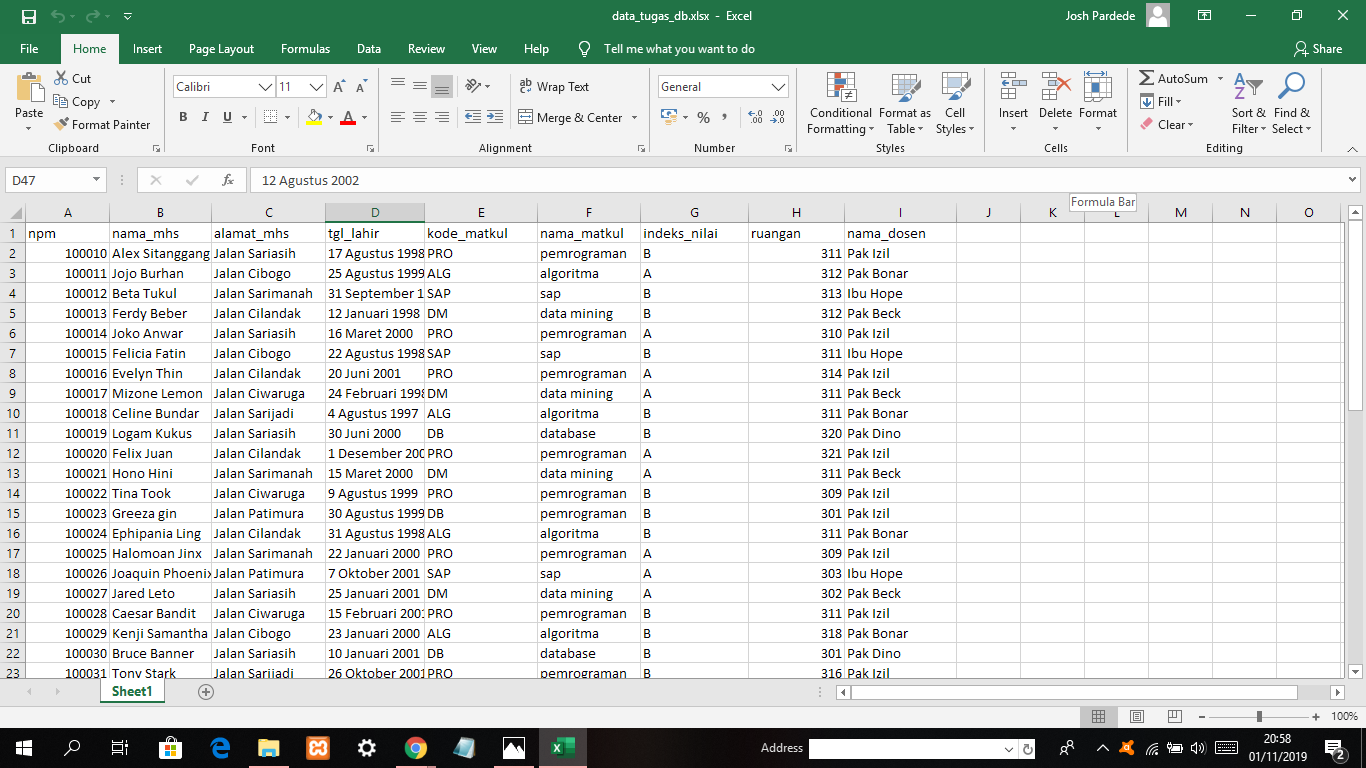
\includegraphics[scale=0.2]{figures/data.png}
    \caption{\textit{Tabel data Mahasiswa}}
    \end{center}   
    \end{figure}
\item[2]Sign in ke dalam website Oracle APEX online Dan klik Request A Workspace.

  
    

\item[3]Isikan data diri anda seperti nama,email,dan workspace.
 \begin{figure}[!htbp]
    \begin{center}
    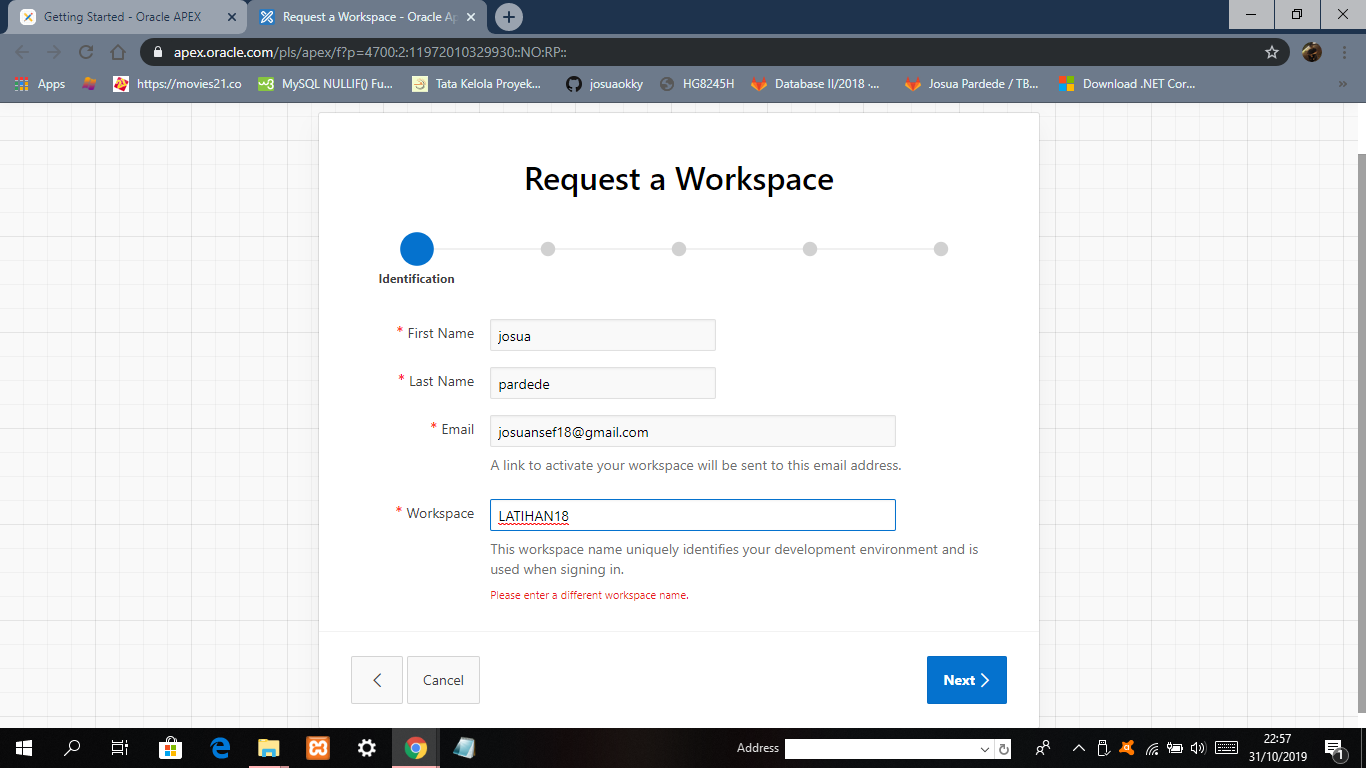
\includegraphics[scale=0.2]{figures/requestworkspace.png}
    \caption{\textit{Isi Data Diri}}
    \end{center}   
    \end{figure}
  
        
\item[4]Centang apakah anda pernah melakukan hal tersebut pada tampilan tersebut setelah itu klik next.  

   
        

\item[5]Isikan pada kolom tersebut data yang diperlukan atau hanya untuk memenuhi kebutuhan survey, lalu klik next.

 



\item[6] Centang Accept, lalu klik next.

 



\item[7]Berikutnya, untuk mengkonfirmasi apakah user ini adalah Anda, klik next.





\item[8] Klik Finish, lalu periksa email anda.

  



\item[9] Selamat Workspace anda telah di Acc lalu klik continue.





\item[10] Workspace Anda telah dibuat, lakukan sign pada website Oracle APEx Online dengan email Anda sebagai username dan password anda.

  



\item[11] Setelah sign in dan masuk ke menu database oracle APEX, klik App Bulider .

 



\item[12] Klik create.





\item[13]Create New App setelah itu pilih From A File.





\item[14]Cari dan drag file .xlsx excel data mahasiwa  yang sebelumnya tadi dibuat ke tampilan From A file





\item[15] Scroll ke bawah lalu lakukan pen-setting-an Table Owner,Table Name,Error Table Name, dan Primary Keys.

 



\item[16] lakukan Load data.
 \begin{figure}[!htbp]
    \begin{center}
    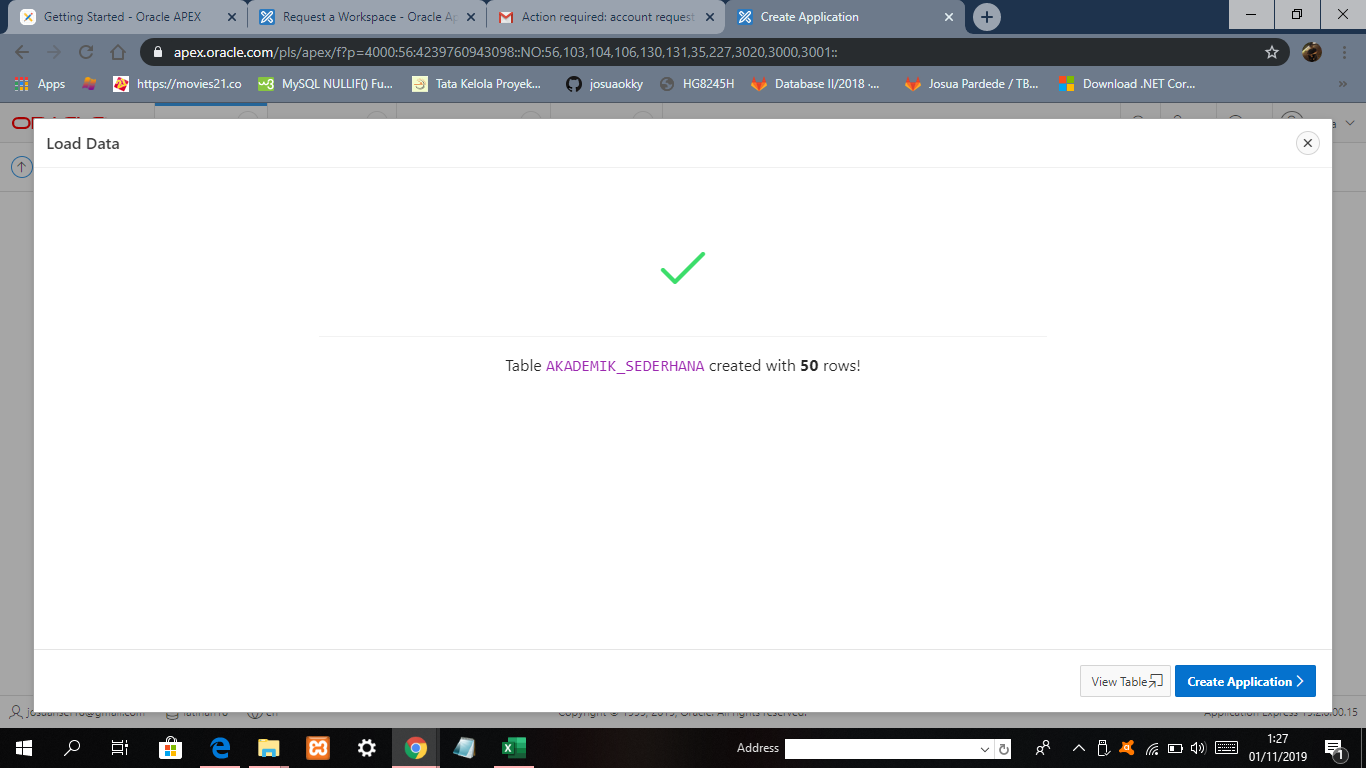
\includegraphics[scale=0.2]{figures/laodeddata.png}
    \caption{\textit{Load Data}}
    \end{center}   
    \end{figure}




\item[17] Kemudian, scroll kebawah dan pastikan semua telah selesai dan fix dan siap untuk dibuat aplikasinya dan Create Application. 
 \begin{figure}[!htbp]
    \begin{center}
    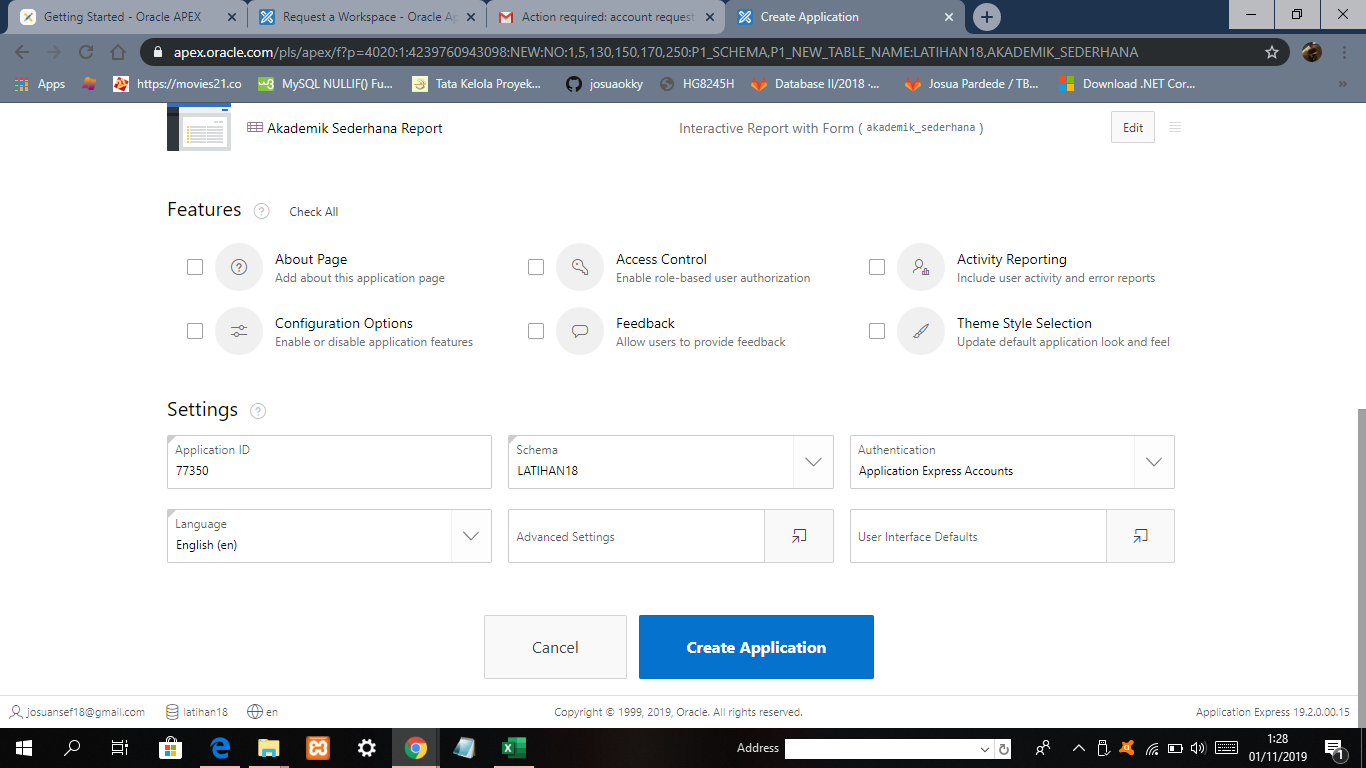
\includegraphics[scale=0.2]{figures/createapp2.png}
    \caption{\textit{Create Application}}
    \end{center}   
    \end{figure}



\item[18] Kemudian Run Application.

 




\item[19]Masukkan username dan password.



\item[20]akan ada tampilan aplikasi dari Aplication Expressnya yang didalamnya ada tabel data mahasiswa.
 \begin{figure}[!htbp]
    \begin{center}
    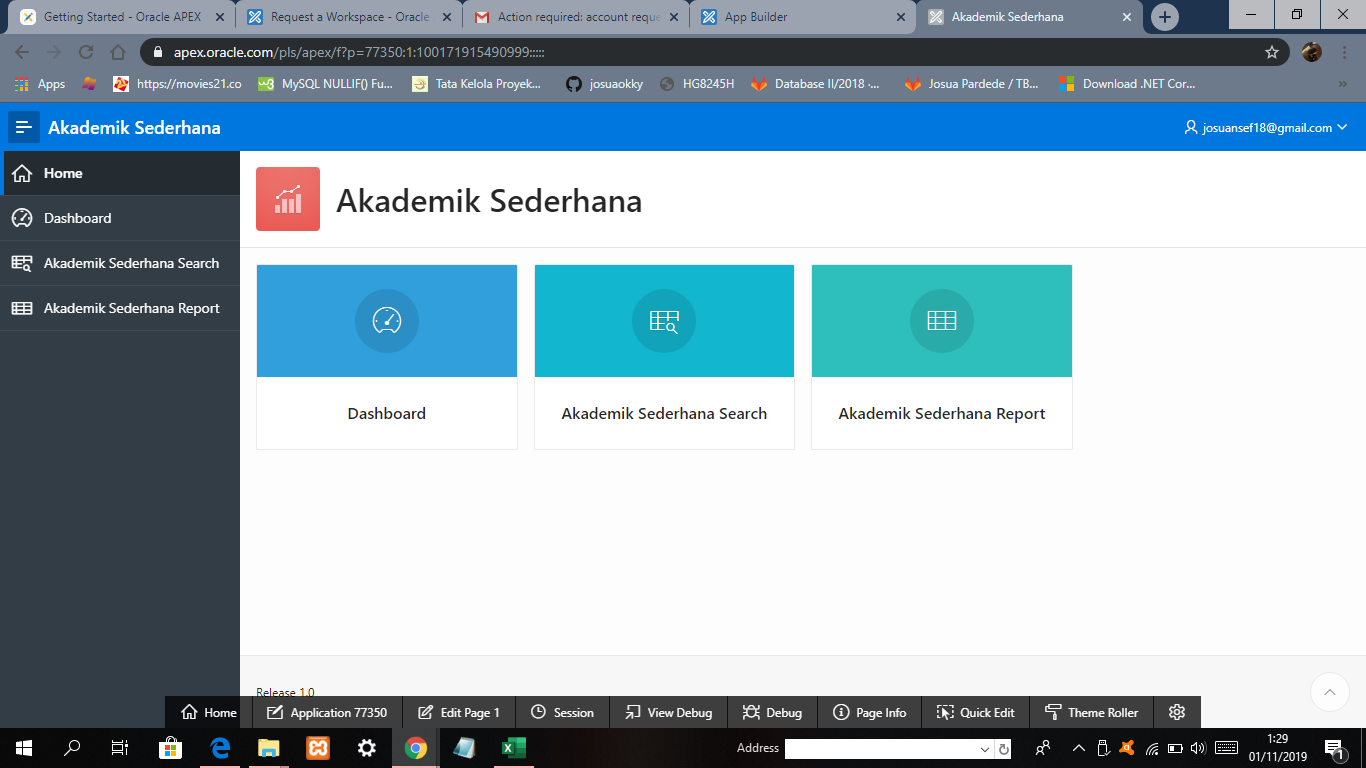
\includegraphics[scale=0.2]{figures/dashboard.png}
    \caption{\textit{Menu Aplikasi Oracle APEX}}
    \end{center}   
    \end{figure}

 



\item[21]Tabel data mahasiswa ada pada pilihan menu Akademik Sederhana di Dashboard.
 \begin{figure}[!htbp]
    \begin{center}
    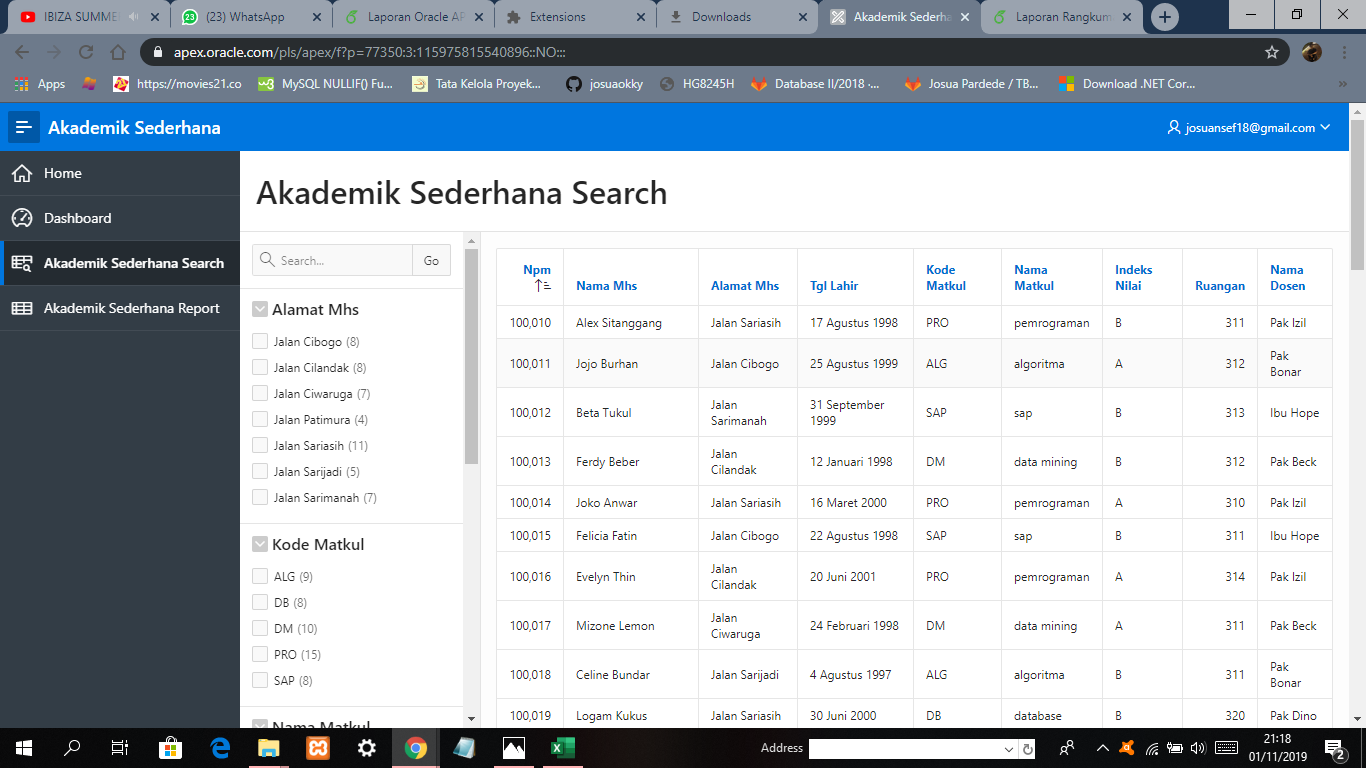
\includegraphics[scale=0.2]{figures/datafile.png}
    \caption{\textit{Data Mahasiswa}}
    \end{center}   
    \end{figure}
    
\item[22]Berikut adalah link Login, username dan password untuk masuk ke Aplikasi Database Oracle Apex dengan nama AKADEMIK SEDERHANA, yang telah dibuat tadi.
link : https://apex.oracle.com/pls/apex/f?p=77350:LOGIN_DESKTOP:116049826285267:::::
username : josuansef18@gmail.com
password : Bandung2020

   

\end{enumerate}
